% !TeX root = ../TFG_LaTeX.tex
\section{Punts fixos i Teorema de Denjoy-Wolff}

\begin{adjustwidth}{1cm}{1cm}

Una vegada estudiades les transformacions de Möbius i els automorfismes del disc unitat, és natural preguntar-se què ocorre quan una d'aquestes aplicacions s'itera repetidament. És a dir, donada una funció $f : \mathbb{D} \to \mathbb{D}$, podem considerar les seues iterades $f^n$ i analitzar el comportament de les òrbites dels punts del disc. En aquest context, els punts fixos tenen un paper essencial, ja que sovint determinen cap a on tendeixen les iterades i permeten classificar la dinàmica de la transformació.

En el cas de les transformacions de Möbius, l'estudi dels punts fixos és especialment manejable, perquè aquests es poden calcular de manera explícita resolent una equació de segon grau. La seua localització, dins del disc, en la frontera o fora d'ell, permet distingir diferents tipus de comportament. Així, els punts fixos no sols donen informació local sobre la funció, sinó que també permeten entendre la seua acció global sobre el pla complex ampliat o sobre el disc unitat.

Aquest estudi culmina amb el Teorema de Denjoy-Wolff, que descriu el comportament asimptòtic de les iterades d'una aplicació holomorfa del disc unitat en si mateix. En aquesta secció ens centrarem en el cas particular de les transformacions de Möbius, on el teorema pot demostrar-se de manera explícita mitjançant el càlcul de punts fixos, i la classificació de les transformacions. D'aquesta manera, obtindrem una descripció concreta del punt cap al qual convergeixen les iterades en cadascun dels casos possibles.

Per al Teorema de Denjoy-Wolff i la seua relació amb la iteració de funcions holomorfes del disc, es pot consultar \cite[Cap. 5]{shapiro}. Per a una perspectiva més general de la dinàmica holomorfa i dels punts fixos, vegeu també \cite{milnor}.


\begin{subsection}{Punts fixos de les transformacions de Möbius}

\begin{definicio}
    Siga $f:\mathbb{C}\to \mathbb{C}$ una funció qualsevol. Direm que $z_0\in \mathbb{C}$ és un \textbf{punt fix} de $f$ si $f(z_0)=z_0$. A més, direm que és un \textbf{punt fix de grau n} si $z_0$ és un zero de grau n de $f(z_0)-z_0$. En concret gastarem el terme \textbf{punt fix doble} per a parlar de zeros de grau dos.
\end{definicio}

\begin{nota}
    Hem definit la funció $f$ de $\mathbb{C}$ en $\mathbb{C}$, però naturalment, també podem definir $f:U\to U$. Realment l'únic que és important és que $f(U)\subseteq U$, ja que això és el que permet que hi hagen punts fixos. 
\end{nota}

\begin{exemple}
    La funció $f(z)=3z+2$ té com a punt fix de grau 1 el punt $z=-1$, ja que $f(z)-z=2z+2=2(z+1)$, que s'anul·la en $z=-1$.
\end{exemple}

\begin{definicio}
    Siga $f:U\to U$ una funció qualsevol, i siga $a$ un punt fix de $f$. Direm que $a$ és un punt fix \textbf{atractor} si existeix un entorn $V$ d'$a$ tal que $f(V)\subset V$ i a més, per a tot $z\in V$, $\displaystyle\lim_{n\to\infty}f^n(z)=a$, on $f^n$ denota la composició de $f$ amb ella mateixa $n$ voltes, és a dir, $f^n=f\circ f\circ \dots \circ f$. En canvi, direm que $a$ és un punt fix \textbf{repulsor} si existeix un entorn $V$ tal que per a tot $z\in V\backslash\{a\}$ existeix un $n\geq 1$ tal que $f^n(z)\notin V$. Per últim, direm que $a$ és un punt fix \textbf{neutre} si no és ni atractor ni repulsor.
\end{definicio}

\begin{proposicio}
    Existeix una caracterització de punt fix atractor, repulsor i neutre en el cas que $f: U\to U$ siga a més, holomorfa.

    Siga $a$ un punt fix de $f$ i considerem $\lambda=f'(a)$, al qual anomenem \textbf{multiplicador de $f$}. Aleshores:
    \begin{equation}
        \begin{aligned}
            |\lambda|<1 &\text{ si i només si } a \text{ és un punt fix atractor},\\
            |\lambda|=1 &\text{ si i només si } a \text{ és un punt fix neutre},\\
            |\lambda|>1 &\text{ si i només si } a \text{ és un punt fix repulsor}.
        \end{aligned}
        \label{caract_pf_atr_neu_rep}
    \end{equation}

    Aquesta informació i altra relacionada amb ella es pot extraure de \cite[pp. 45,76]{milnor}
\label{prop_caract_pf}
\end{proposicio}
    
A més, encara que no entra en el domini en la definició que hem donat, també podem estudiar el punt $\infty$.

\begin{definicio}
    Si considerem $f:\mathbb{C}^*\to \mathbb{C}^*$, direm que el punt $\infty$ és un punt fix de $f$ si $f(\infty)=\infty$.
\end{definicio}

\begin{proposicio}
    Es té que $\infty$ és un punt fix de $f:\mathbb{C}^*\to \mathbb{C}^*$ si i sols si $0$ és un punt fix de $g:\mathbb{C}^*\to \mathbb{C}^*$, donat per $g(u)=\frac{1}{f(1/u)}$.
    \label{punt_fix_inf}
\end{proposicio}

\begin{proof}
    Per l'aritmètica de $\mathbb{C}^*$, vista en la Definició \ref{pla_complex_ampliat}, tenim que
    \[
        g(0)=\frac{1}{f(1/0)}=\frac{1}{f(\infty)}=\frac{1}{\infty}=0.
    \]
\end{proof}

\begin{nota}
    Així, podem ampliar la Proposició \ref{prop_caract_pf} si $\infty$ és punt fix de $f:\mathbb{C}^*\to \mathbb{C}^*$, considerant que $0$ és punt fix de $g$, donada per $g:\mathbb{C}^*\to \mathbb{C}^*$, $g(u)=\frac{1}{f(1/u)}$.
\end{nota}

\begin{definicio}
    Siga $f:\mathbb{C}^*\to \mathbb{C}^*$ una funció qualsevol, i siga $z_0\in \mathbb{C}^*$. Anomenarem \textbf{òrbita de $z_0$} al conjunt $\{z_0, f(z_0),f^2(z_0),\dots\}$.
\end{definicio}

\begin{proposicio}
    Siga $f:\mathbb{D}\to \mathbb{D}$ una funció holomorfa distinta de la identitat. Aleshores $f$ té un punt fix com a molt. A més, tampoc pot tindre un punt fix doble.
    \label{max_1_punt_fix_en_D}
\end{proposicio}

\begin{proof}
    Siguen $a,b\in \mathbb{D}$ dos punts fixos de $f$, és a dir, que $f(a)=a$ i $f(b)=b$. Suposem per reducció al absurd que $a\neq b$.

    Siga l'automorfisme $\phi(z)=e^{i\theta}\varphi_a(z)$ on $0\leq\theta<2\pi$ i on $\varphi_a$ és l'automorfisme definit en la Definició \ref{varphi_a}. Per tant, $\phi^{-1}(w)=\varphi_a(e^{-i\theta}w)$ (Proposició \ref{inv_phi}) també és automorfisme pel Teorema \ref{bij_holo_te_inv_holo}. Aleshores, per com hem definit $\varphi_a$, tenim que $\varphi_a(0)=a$, i siga $c\in \mathbb{D}$ tal que $\varphi_a(b)=c$. Notem que $c\neq 0$ perquè $a\neq b$ i perquè $\varphi_a(a)=0$, i ja no hi ha més zeros perquè $\varphi_a$ és un automorfisme.

    Ara, si definim $g:=\varphi_a\circ f\circ \varphi^{-1}_a$, aquesta $g$ fixa el punt $0$ i el punt $c$. Efectivament, 
    \begin{equation}
        \begin{aligned}
            g(0) =& \varphi_a(f(\varphi^{-1}_a(0)))=\varphi_a(f(a))=\varphi_a(a)=0, \\
            g(c) =& \varphi_a(f(\varphi^{-1}_a(c)))=\varphi_a(f(b))=\varphi_a(b)=c.
        \end{aligned}
    \end{equation}

    Ara bé, com $g:\mathbb{D}\to \mathbb{D}$ és holomorfa i fixa el $0$, podem aplicar el Lema de Schwarz (Lema \ref{LemaSchwarz}) i obtenir que per a tot $z\in \mathbb{D}$, $|g(z)|\leq|z|$, però a més, com $g(c)=c$, sent $c\neq 0$, obtenim també que $g(z)=z$, i per tant $g$ és la identitat. Així doncs, $f=\varphi^{-1}_a\circ g\circ\varphi_a=\varphi^{-1}_a\circ\varphi_a=id_{\mathbb{D}}$, i això contradiu l'enunciat. Per tant, l'error ve de suposar que $a$ i $b$ són distints. Així, $f$ no pot tindre més d'un punt fix.

    La prova de que no pot tindre un punt fix doble és molt similar. Suposem que $a\in \mathbb{D}$ és un punt fix doble, i prenem l'automorfisme $\varphi_a$ d'abans. Aleshores $g:=\varphi_a\circ f\circ \varphi^{-1}_a$ torna a complir que $g(0)=0$, i a més $0$ és punt fix doble. Considerant el desenvolupament de Taylor de la funció $g(z)$ centrada en 0, tenim que 
    \[
        g(z)=g(0)+g'(0)z+\dots, \; \text{ i per tant } \; g(z)-z=(g'(0)-1)z+\dots.
    \]
    Com $0$ és un zero doble de $g(z)-z$, això significa que el seu desenvolupament de Taylor en 0 no té terme lineal, i per tant $g'(0)=1$. D'eixa forma, el Lema \ref{LemaSchwarz_2} ens diu que si $|g'(0)|=1$, aleshores $g(z)=\lambda z$, sent el mòdul de $\lambda$ 1, però com $g'(0)=1$, aleshores $\lambda=1$ i $g$ és la identitat, cosa que implica que $f$ també es la identitat, arribant a una contradicció.
\end{proof}

\begin{nota}
    Combinant la Proposició \ref{max_1_punt_fix_en_D} i el Teorema del Punt Fix de Brouwer (Teorema \ref{brouwer}) obtenim que, si tenim una funció $f:\overline{\mathbb{D}}\to\overline{\mathbb{D}}$ holomorfa i distinta de la identitat, aleshores les úniques possibilitats són les següents:
    \begin{enumerate}
        \item $f$ té exactament un punt fix, que pot estar en $\mathbb{D}$ o en $\partial \mathbb{D}$.
        \item $f$ té més d'un punt fix, i tots ells, excepte potser un, estan en $\partial \mathbb{D}$.
    \end{enumerate}
    \label{nota_ubicacio_pf_1}
\end{nota}

\begin{nota}
    Anem a denotar com $TM(\mathbb{D})$ al conjunt de transformacions de Möbius que quan les restringim a $\mathbb{D}$ van a parar a $\mathbb{D}$. Normalment parlarem directament de $\varphi:\mathbb{D}\to \mathbb{D}$, mentre es tinga clar que és una restricció.
    \label{notacio_TM}
\end{nota}

\begin{corolari}
    Si $\varphi:\mathbb{D}\to \mathbb{D}$ és una transformació de Möbius que no té punts fixos en $\mathbb{D}$, aleshores es pot estendre contínuament a $\tilde{\varphi}:\overline{\mathbb{D}}\to\overline{\mathbb{D}}$ i $\tilde{\varphi}$
    necessàriament té almenys un punt fix en $\partial \mathbb{D}$.
    \label{extensio_cont_TM}
\end{corolari}

\begin{proof}
    L'avantatge que tenim ara és que com $\varphi$ és holomorfa en $\mathbb{D}$ i a més $\varphi(\mathbb{D})\subseteq \mathbb{D}$, aleshores no pot tindre un pol en $\overline{\mathbb{D}}$, perquè si no en acostar-se al pol la funció no estaria fitada, però $|\varphi(z)|\leq 1$. Aleshores podem estendre $\varphi$ a $\tilde{\varphi}$ contínuament  a $\overline{\mathbb{D}}$, i per continuïtat, $\tilde{\varphi}(\overline{\mathbb{D}})\subseteq \overline{\mathbb{D}}$. Així, aplicant el Teorema del Punt Fix de Brouwer (Teorema \ref{brouwer}), $\tilde{\varphi}$ té almenys un punt fix en $\partial \mathbb{D}$.
\end{proof}

\begin{nota}
    En el corol·lari anterior hem denotat a l'estensió de $\varphi$ com $\tilde{\varphi}$, però a partir d'ara, per simplicitat, es seguirà denotant com $\varphi$.
\end{nota}

\begin{proposicio}
    Si $\varphi:\mathbb{C}^*\to \mathbb{C}^*$, $\varphi(z)=\frac{az+b}{cz+d}$ és una transformació de Möbius distinta de la identitat, aleshores  $\varphi$ fixa o bé un punt doble o bé dos punts. 
    \label{transformació_moeb_fix}
\end{proposicio}

\begin{proof}
    Si $z$ és un punt fix de $\varphi$, podem escriure 
    \[
        \varphi(z)=\frac{az+b}{cz+d}=z \iff az+b=cz^2+dz\iff cz^2+(d-a)z-b=0.
    \]

    Així, si $c\neq 0$, com a molt hi ha dos punts fixos, ja que pot passar que la solució de l'equació siga doble i en eixe cas sols hi ha un punt fix, però sempre són punts fixos complexos. Ara bé, si $c=0$, aleshores tenim que la transformació sempre fixa el punt a l'infinit, i a més també té punt fix complex en el cas que $a\neq d$. Si $a=d$, aleshores fixa tots els punts, perquè en eixe cas $\varphi$ és la identitat, ja que l'equació implica $b=0$.
\end{proof}

\begin{nota}
    Concretament, i seguint amb la notació de la demostració anterior, si $c\neq 0$, tenim que els punts fixos de $\varphi$ són
    \[
        z_1= \frac{(a-d)+\sqrt{(a-d)^2+4bc}}{2c}, \qquad 
        z_2= \frac{(a-d)-\sqrt{(a-d)^2+4bc}}{2c},
    \]
    i serà un punt doble, $\frac{(a-d)}{2c}$ quan $(a-d)^2=-4bc$.

    A més, si $c=0$ i $a\neq d$, aleshores l'únic punt fix complex és $z=\frac{b}{d-a}$.
    \label{punts_fixos_explicits}
\end{nota}

\begin{nota}
    Connectant ara la Nota \ref{nota_ubicacio_pf_1} i la Proposició \ref{transformació_moeb_fix}, tenim que si $\varphi:\overline{\mathbb{D}}\to\overline{\mathbb{D}}$ és una transformació de Möbius distinta a la identitat, aleshores poden passar quatre casos:
    \begin{enumerate}
        \item  $\varphi$ té un únic punt fix i està en $\mathbb{D}$.
        \item $\varphi$ té un únic punt fix i està en $\partial \mathbb{D}$
        \item $\varphi$ té dos punts fixos, un en $\mathbb{D}$ i l'altre en $\partial \mathbb{D}$.
        \item $\varphi$ té dos punts fixos, els dos en $\partial \mathbb{D}$.
    \end{enumerate}
    \label{possibilitats_pf}
\end{nota}

Ara, amb un esquema més clar de com funcionen els punts fixos de les transformacions de $TM(\mathbb{D})$, passem amb la classificació.

\begin{definicio}
    Podem classificar les funcions de $TM(\mathbb{D})\backslash\{\operatorname{id_{\mathbb{C}^*}}\}$ (Nota \ref{notacio_TM}) en tres grups:
    \leavevmode
    \begin{enumerate}
        \item Direm que $\varphi\in TM(\mathbb{D})$ és \textbf{parabòlica} si té un punt fix doble en $\partial\mathbb{D}$.
        \item Direm que $\varphi\in TM(\mathbb{D})$ és \textbf{hiperbòlica} si té un punt fix atractor en $\partial\mathbb{D}$, i el altre punt fix fora de $\mathbb{D}$, estant aquest en $\partial \mathbb{D}$ si i només si $\varphi$ és un automorfisme de $\mathbb{D}$.
        \item Direm que $\varphi\in TM(\mathbb{D})$ és \textbf{loxodròmica} si té un punt fix en $\mathbb{D}$ i altre punt fix fora de $\mathbb{D}$. Si a més $\varphi$ és un automorfisme, direm que és \textbf{elíptica}.
    \end{enumerate}
    \label{classificació_TM}
\end{definicio}

\begin{nota}
    Notem que la definició anterior és exhaustiva. No pot passar que, sent $\varphi:\mathbb{C}^*\to \mathbb{C}^*$ tal que $\varphi$ envia $\mathbb{D}$ en ell mateix, i no siga la identitat, hi haja un únic punt fix en $\mathbb{D}$ ni fora de $\overline{\mathbb{D}}$.
    
    Si hi haguera un únic punt fix i estiguera fora de $\overline{\mathbb{D}}$, això contradiria el Teorema del Punt Fix de Brouwer (Teorema \ref{brouwer}) en $\overline{\mathbb{D}}$.

    Si hi haguera un únic punt fix i estiguera en $\mathbb{D}$, aquest seria doble per la Proposició \ref{transformació_moeb_fix}, i això contradiria la Proposició \ref{max_1_punt_fix_en_D}. 
\end{nota}

\begin{exemple}[Transformació parabòlica]
    La transformació $\varphi(z)=\frac{z+1}{3-z}$, $\varphi\in TM(\mathbb{D})$ és parabòlica. En efecte, segons com ens diu la Nota \ref{punts_fixos_explicits} el punt $z=\frac{1-3}{-2}=1\in\partial \mathbb{D}$ és punt fix doble, que a més és neutre perquè $\varphi'(z)=\frac{4}{(3-z)^2}$ i per tant $\varphi'(1)=1$. Gràficament,

    \begin{figure}[H]
        \centering
        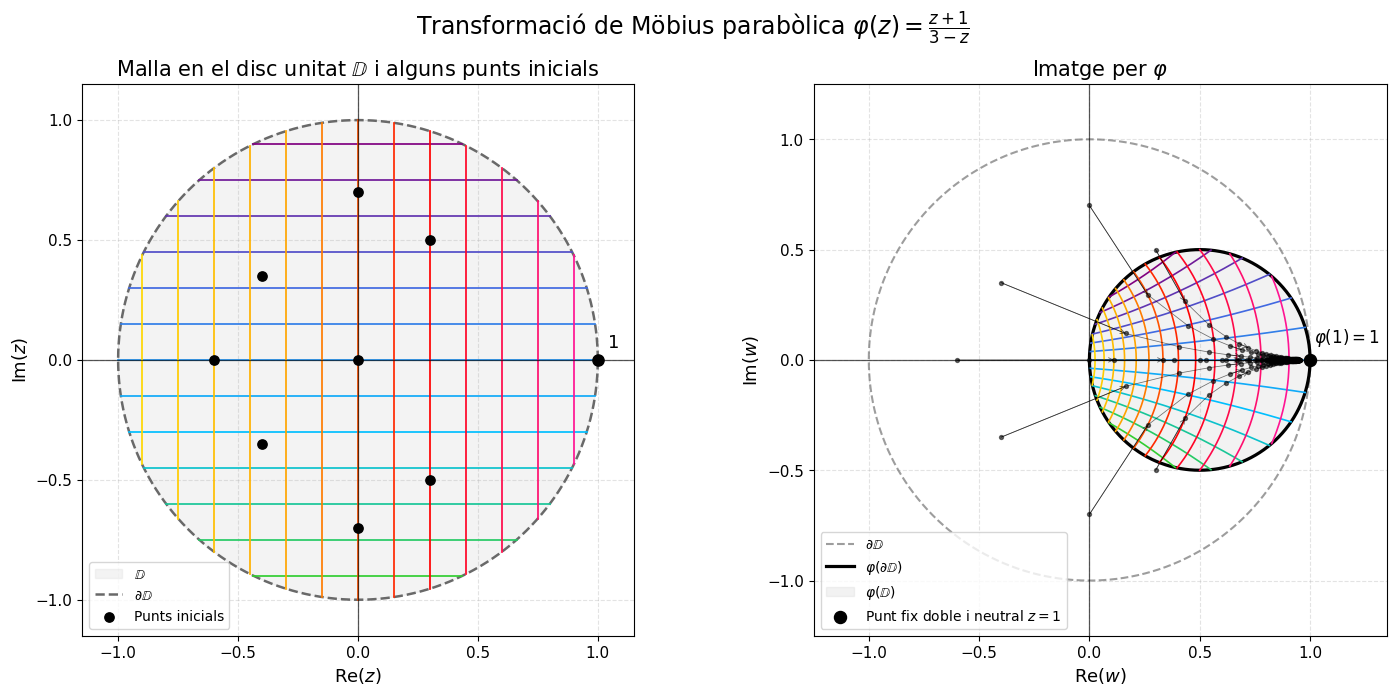
\includegraphics[width=0.9\textwidth]{pictures/funcionparabolica3.png}
        \begin{adjustwidth}{1cm}{1cm}
        \caption{Imatge de $\varphi(z)=\frac{z+1}{3-z}$ per a $z\in \mathbb{D}$.}
        \label{fig:parabolica} 
        \end{adjustwidth}
    \end{figure}

    \begin{nota}
        Un detall a comentar és que, en la imatge pareix que el punt fix 1 siga atractor, però no ho és. Açò és degut a que sols hem vist que els punts de dins de $\mathbb{D}$ s'acosten a $1$, però necessitem també, per la definició d'atractor, que hi haja un entorn $U$ de $1$ tal que $\varphi(U)\subset U$, (i recordem que $\varphi$ en general està definida en $\mathbb{C}^*$). Ara bé, si prenem $U$ la bola centrada en 1 de radi arbitràriament menut $\varepsilon>0$ i prenem $z_0=1+\delta \in U$, on $\frac{\varepsilon}{1+\frac{\varepsilon}{2}}<\delta<2$, aleshores $\varphi(z_0)=\frac{2+\delta}{2-\delta}=1+\frac{\delta}{1-\frac{\delta}{2}}>1+\varepsilon$, ja que 
        \[
            \frac{\delta}{1-\frac{\delta}{2}}>\varepsilon \iff \delta>\varepsilon-\frac{\varepsilon\delta}{2} \iff \delta>\frac{\varepsilon}{1+\frac{\varepsilon}{2}}
        \] 
        cosa que és certa, i per tant $\varphi(z_0)\notin U$. Per tant, en aquest sentit, la imatge és un poc enganyosa.
    \end{nota}

\end{exemple}

\begin{exemple}[Transformació hiperbòlica automorfa en $\mathbb{D}$]
    La transformació $\varphi(z)$ $=\frac{2z+1}{z+2}$, $\varphi\in TM(\mathbb{D})$ és hiperbòlica i a més és un automorfisme sobre $\mathbb{D}$. Coherentment amb la definició que hem donat, tenim un punt fix atractor en $\partial \mathbb{D}$, i un altre punt fix en $\partial \mathbb{D}$. Segons la Nota \ref{punts_fixos_explicits}, els punts fixos són
    \[
        z_1=\frac{0+\sqrt{0^2+4\cdot1\cdot1}}{2\cdot1}=1, \qquad z_2=\frac{0-\sqrt{0^2+4\cdot1\cdot1}}{2\cdot1}=-1.
    \]
    Com tenim que $\varphi'(z)=\frac{3}{(z+2)^2}$, el primer és punt fix atractor, ja que $\varphi'(1)=\frac{1}{3}<1$, i el segon és repulsor, ja que $\varphi'(-1)=3>1$.

    Efectivament, ho podem veure en la següent imatge.

    \begin{figure}[H]
        \centering
        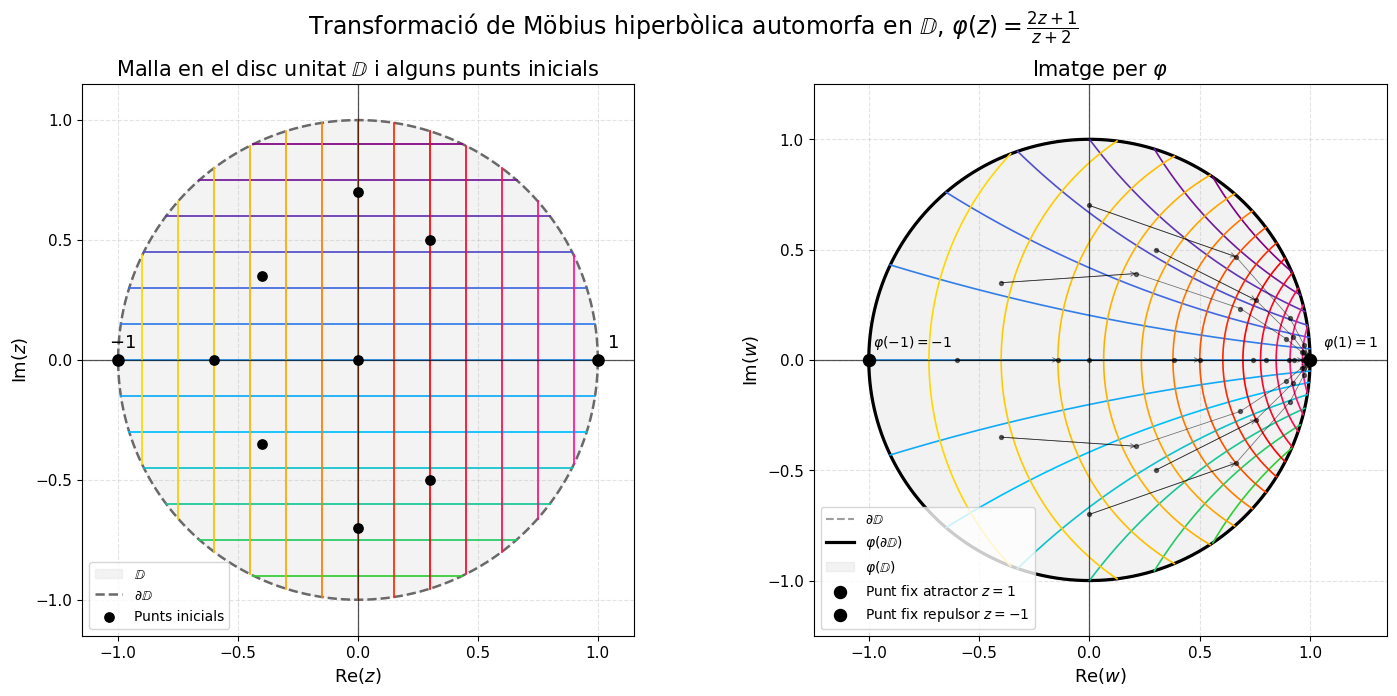
\includegraphics[width=0.9\textwidth]{pictures/funcionhiperbolica1.png}
        \begin{adjustwidth}{1cm}{1cm}
        \caption{Imatge de $\varphi(z)=\frac{2z+1}{z+2}$ per a $z\in \mathbb{D}$.}
        \label{fig:hiperbolica1} 
        \end{adjustwidth}
    \end{figure}

\end{exemple}

\begin{exemple}[Transformació hiperbòlica no automorfa en $\mathbb{D}$]
    La transformació $\varphi(z)$ $=\frac{z+1}{2}$, $\varphi\in TM(\mathbb{D})$ és hiperbòlica però en aquest cas no és un automorfisme sobre $\mathbb{D}$. Coherentment amb la definició que hem donat, tenim un punt fix atractor en $\partial \mathbb{D}$, i un altre punt fix fora de $\overline{\mathbb{D}}$. Segons la Nota \ref{punts_fixos_explicits}, els punts fixos són l'infinit $\infty$ i el punt complex $\frac{1}{2-1}=1$.

    Com tenim que $\varphi'(z)=\frac{1}{2}<1$, el punt fix 1 és atractor.

    Per a vore de quin tipus és el punt fix $\infty$, considerem la funció conjugada $g(u)=\frac{1}{\varphi(1/u)}=\frac{2}{\frac{1}{u}+1}=\frac{2u}{u+1}$. Per tant, $g'(u)=\frac{2}{(u+1)^2}$, i $g'(0)=2>1$. Per tant, el punt $\infty$ és punt fix repulsor de $f$.

    Efectivament, en la següent imatge podem veure que el que passa en $\overline{\mathbb{D}}$.

    \begin{figure}[H]
        \centering
        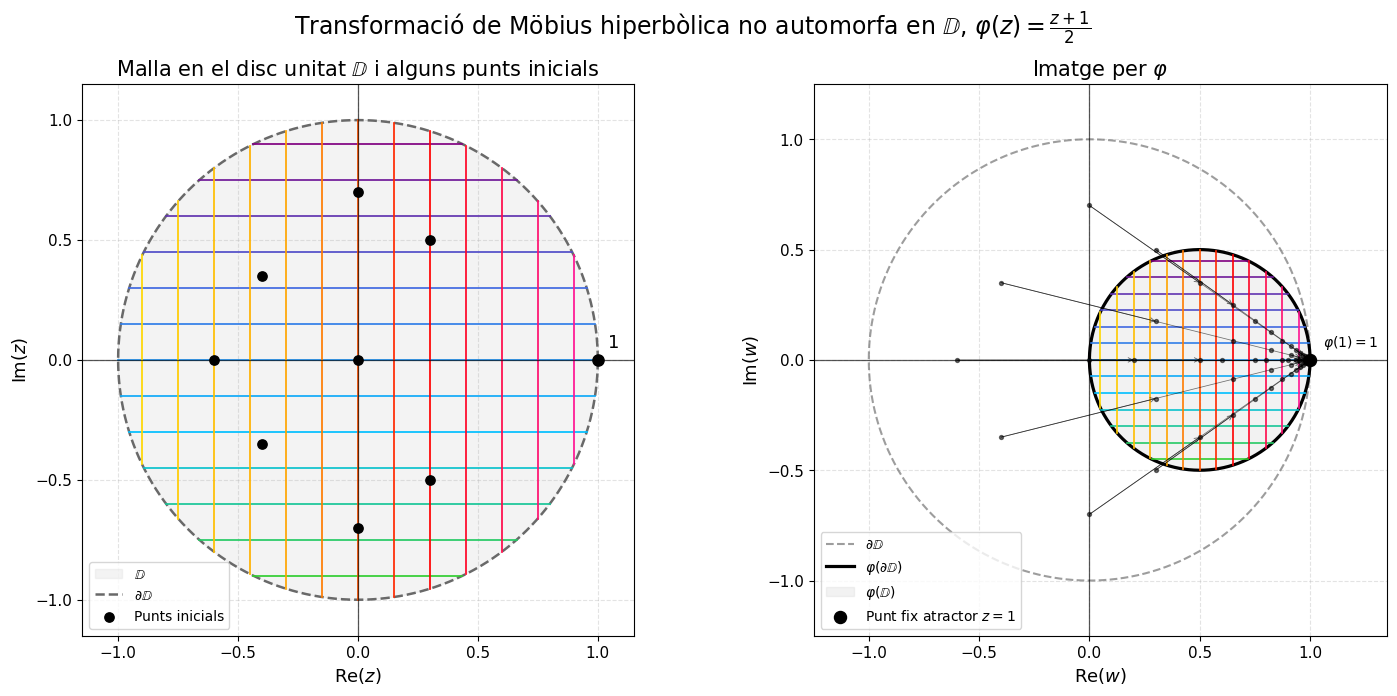
\includegraphics[width=0.9\textwidth]{pictures/funcionhiperbolica2.png}
        \begin{adjustwidth}{1cm}{1cm}
        \caption{Imatge de $\varphi(z)=\frac{z+1}{2}$ per a $z\in \mathbb{D}$.}
        \label{fig:hiperbolica2} 
        \end{adjustwidth}
    \end{figure}

\end{exemple}

\begin{exemple}[Transformació loxodròmica no automorfa]
    La transformació $\varphi(z)$ $=\frac{z}{2}$, $\varphi\in TM(\mathbb{D})$ és loxodròmica i no és un automorfisme sobre $\mathbb{D}$. Coherentment amb la definició que hem donat, tenim un punt fix en $\mathbb{D}$, i un altre punt fix fora de $\mathbb{D}$. Segons la Nota \ref{punts_fixos_explicits}, els punts fixos són l'infinit $\infty$ i el punt complex $\frac{0}{2-1}=0$.

    Com tenim que $\varphi'(z)=\frac{1}{2}<1$, el punt fix 0 és atractor.

    Per a vore de quin tipus és el punt fix $\infty$, considerem la funció conjugada $g(u)=\frac{1}{\varphi(1/u)}=\frac{2}{\frac{1}{u}}=2u$. Per tant, $g'(u)=2$, i $g'(0)=2>1$. Per tant, el punt $\infty$ és punt fix repulsor de $f$.

    Efectivament, en la següent imatge podem veure que el que passa en $\overline{\mathbb{D}}$.

    \begin{figure}[H]
        \centering
        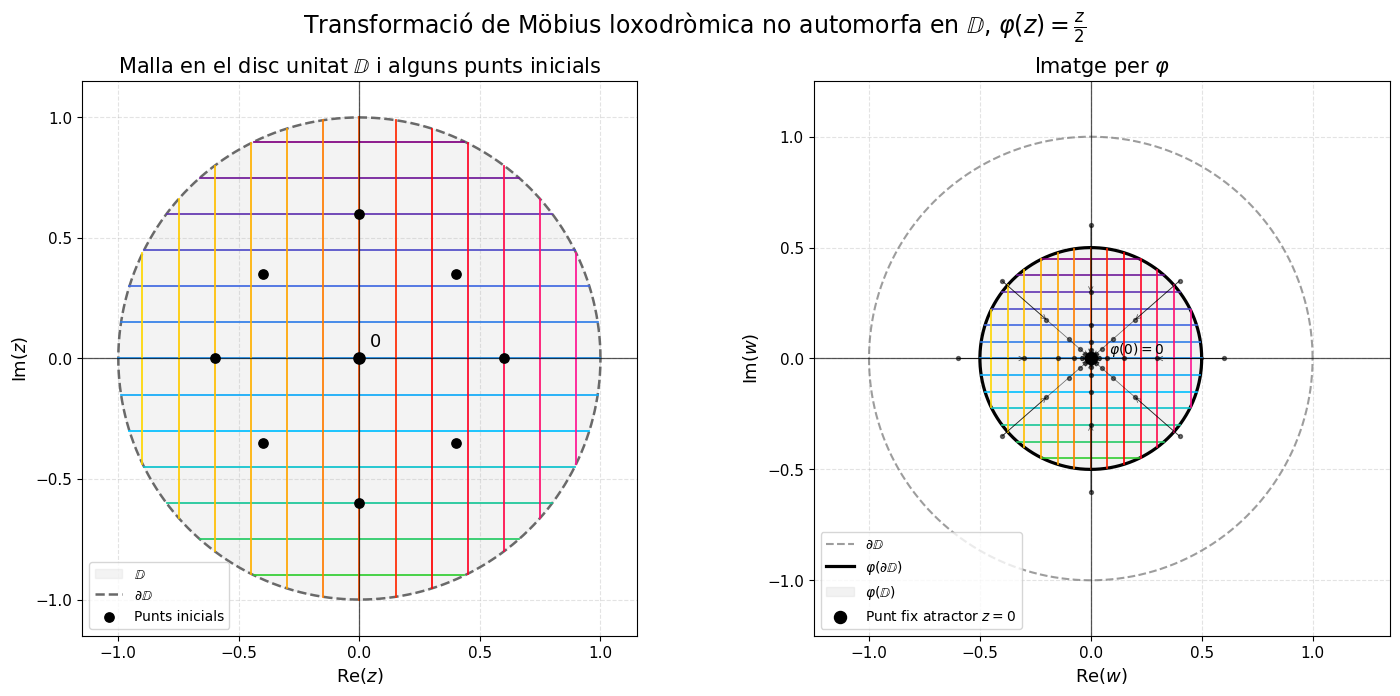
\includegraphics[width=0.9\textwidth]{pictures/funcionloxodromica.png}
        \begin{adjustwidth}{1cm}{1cm}
        \caption{Imatge de $\varphi(z)=\frac{z}{2}$ per a $z\in \mathbb{D}$.}
        \label{fig:loxodròmica} 
        \end{adjustwidth}
    \end{figure}

\end{exemple}

\begin{exemple}[Transformació elíptica]
    La transformació $\varphi(z) = e^{i\pi/2}z$, amb $\varphi\in TM(\mathbb{D})$, és elíptica, és a dir, és loxodròmica i, a més, sobre $\mathbb{D}$ és un automorfisme. Coherentment amb la definició que hem donat, tenim un punt fix en $\mathbb{D}$, i un altre punt fix fora de $\mathbb{D}$. Segons la Nota \ref{punts_fixos_explicits}, els punts fixos són l'infinit $\infty$ i el punt complex $\frac{0}{1-e^{i\pi/2}}=0$.

    Com tenim que $\varphi'(z)=e^{i\pi/2}$ i, per tant, $|\varphi'(z)|=1$, el punt fix 0 és neutre.

    Per a vore de quin tipus és el punt fix $\infty$, considerem la funció conjugada $g(u)=\frac{1}{\varphi(1/u)}=\frac{u}{e^{i\pi/2}}$. Per tant, $g'(u)=\frac{1}{e^{i\pi/2}}$, i $|g'(0)|=1$. Per tant, el punt $\infty$ és punt fix neutre de $f$.

    Efectivament, en la següent imatge podem veure que el que passa en $\overline{\mathbb{D}}$.

    \begin{figure}[H]
        \centering
        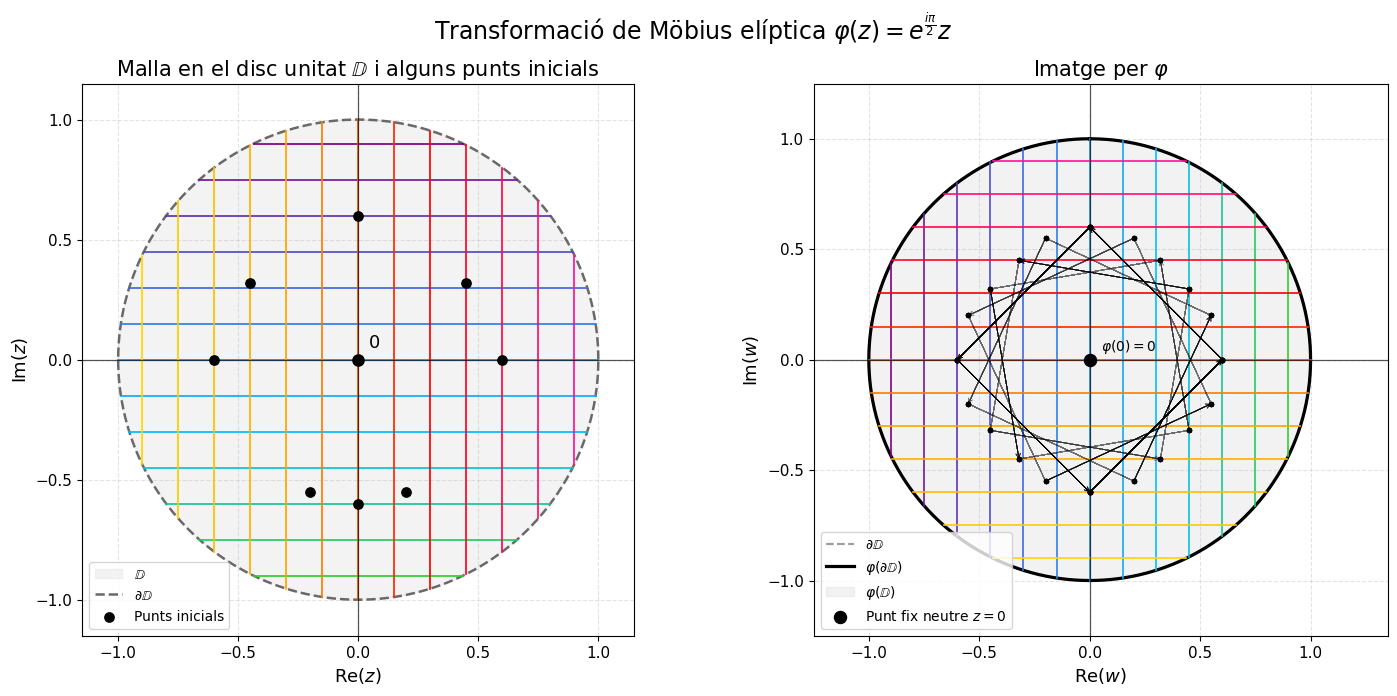
\includegraphics[width=0.9\textwidth]{pictures/funcioneliptica.png}
        \begin{adjustwidth}{1cm}{1cm}
        \caption{Imatge de $\varphi(z)=e^{i\pi/2}z$ per a $z\in \mathbb{D}$.}
        \label{fig:elíptica} 
        \end{adjustwidth}
    \end{figure}

\end{exemple}

\end{subsection}

\begin{subsection}{Teorema de Denjoy-Wolff}

    \begin{teorema}[Denjoy-Wolff]
        Siga $\varphi: \mathbb{D}\to \mathbb{D}$ una funció holomorfa que no és la identitat ni un automorfisme elíptic. Aleshores existeix un punt $\alpha\in \overline{\mathbb{D}}$ tal que $\displaystyle\lim_{n\to\infty}\varphi^n(z)=\alpha$ uniformement sobre subconjunts compactes de $\mathbb{D}$.
    \end{teorema}

    Per a provar el Teorema de Denjoy-Wolff es necessita gastar formes normals i el Lema de Wolff. Açò queda fora de l'abast del que pretén aquest treball. El que farem nosaltres és provar una versió del Teorema de Denjoy-Wolff només per a transformacions de Möbius, ja que és molt més coherent amb el que estem fent i és molt interessant. No obstant això, abans d'enunciar-lo provarem alguns resultats que farem servir en la prova d'aquest teorema.

    %\begin{lema}
    %    Siga $\varphi\in TM(\mathbb{D})$ una transformació de Möbius que no és un automorfisme de $\mathbb{D}$, i siga $K\subset \mathbb{D}$ un subconjunt compacte. Aleshores tenim que existeix un $k\in(0,1)$ de forma que 
    %    \[
    %        \rho(\varphi(z),\varphi(w))\leq k\rho(z,w)
    %    \]
    %    per a tot $z,w\in K$.
    %   \label{lema_dw}
    %\end{lema}

    %\begin{proof}
    %    Comencem definint la funció 
    %    \[
    %        \Phi:K\times K \to \mathbb{R}, \qquad \Phi(z,w)= \begin{cases}
    %            \begin{aligned}
    %                \frac{\rho(\varphi(z),\varphi(w))}{\rho(z,w)} & \text{ si } z\neq w \\
    %                \frac{|\varphi'(z)|(1-|z|^2)}{1-|\varphi(z)|^2} & \text{ si } z=w
    %            \end{aligned}
    %        \end{cases}.
    %    \]

    %    És evident que la funció és contínua en els punts $(z,w)\in K\times K$ tal que $z\neq w$, ja que la mètrica pseudohiperbòlica és contínua. Estudiem doncs la continuitat dels punts de la forma $(z,z)\in K\times K$.

    %    Tenim que 
    %    \[
    %        \frac{\rho(\varphi(z),\varphi(w))}{\rho(z,w)}=\frac{\left|\frac{\varphi(z)-\varphi(w)}{1-\overline{\varphi(w)}\varphi(z)}\right|}{\left|\frac{z-w}{1-\overline{w}z}\right|}=\left|\frac{\varphi(z)-\varphi(w)}{z-w}\right|\left|\frac{1-\overline{w}z}{1-\overline{\varphi(w)}\varphi(z)}\right|,
    %    \]
    %     i per tant, fixant ara $z\in K$ i prenent el límit quan $w$ tendeix a $z$, obtenim que, pels càlculs fets en l'equació (\ref{eq_limit_met_pseudohip}), 
    %    \begin{equation}
    %            \lim_{w\to z}\Phi(w,z)=\lim_{w\to z}\frac{\rho(\varphi(z),\varphi(z))}{\rho(z,w)}=|\varphi'(z)|\frac{1-|z|^2}{1-|\varphi(z)|^2}=\Phi(z,z).
    %        \label{eq_lema_dw}
    %    \end{equation}

    %    Aleshores, efectivament la funció $\Phi$ és contínua en $K\times K$, compacte per ser producte de compactes. Per tant, existeix un punt $(z_0,w_0)\in K\times K$ de forma que $\Phi(z,w)\leq\Phi(z_0,w_0)$ per a tot $z,w\in K$. Anem a separar casos depenent de si $z_0\neq w_0$ o si $z_0=w_0$. Comencem amb el primer cas.

    %    Ara, com $\varphi$ no és un automorfisme del disc, apliquem el Lema de Schwarz-Pick (Lema \ref{schwarz_pick}) per a poder afirmar que 
    %    \[
    %        \rho(\varphi(z_0),\varphi(w_0))<\rho(z_0,w_0).
    %    \]
    %    Com $z_0\neq w_0$, això ho podem reescriure com 
    %    \[
    %        \Phi(z_0,w_0)=\frac{\rho(\varphi(z_0),\varphi(w_0))}{\rho(z_0,w_0)}<1.
    %    \]
    %    Conseqüentment, per a tot $z,w\in K$ tenim que
    %    \[
    %         \Phi(z,w)\leq\Phi(z_0,w_0)< 1,
    %    \]

     %   Per altra banda, suposem ara que $z_0=w_0$.

     %   Gastant de nou que $\varphi$ no és un automorfisme del disc, apliquem el Lema de Pick (Lema \ref{pick}) per a poder afirmar que 
     %   \[
     %       \Phi(z_0,z_0)=|\varphi'(z_0)|\frac{1-|z_0|^2}{1-|\varphi(z_0)|^2}<\frac{1-|z_0|^2}{1-|\varphi(z_0)|^2}\frac{1-|\varphi(z_0)|^2}{1-|z_0|^2}=1.
     %   \]
     %   Així, tenim que per a tot $z,w\in K$, 
     %   \[
     %       \Phi(z,w)\leq\Phi(z_0,z_0)<1
    %    \]
    %    Per tant, en qualsevol cas hem arribat a que $\Phi(z,w)<1$.
    %
    %    Reescrivint això per a tot $z,w\in K$ amb $z\neq w$, obtenim que
    %    \[
    %        \rho(\varphi(z),\varphi(w))<\rho(z,w).
    %    \]
    %    A més, si $z=w$ tenim que $\rho(z,w),\rho(\varphi(z),\varphi(w))=0$, i per tant, en qualsevol cas existeix $k\in (0,1)$ de forma que, per a tot $z,w\in K$, 
     %   \[
    %        \rho(\varphi(z),\varphi(w))\leq k\rho(z,w).
    %    \]

    %\end{proof}

    %\begin{nota}
    %    Notem que en (\ref{eq_lema_dw}), hem agafat $\Phi(z,w)$ sense pèrdua de generalitat, ja que com la mètrica pseudohiperbòlica $\rho$ és simètrica per ser mètrica, podriem haver agafat també $\Phi(w,z)$.
    %\end{nota}

    \begin{nota}
        Recordem que si $u,v\in \mathbb{R}$, aleshores
        \begin{equation}
            \tan(u+v)=\frac{\tan(u)+\tan(v)}{1-\tan(u)\tan(v)}, \qquad \tan(u-v)=\frac{\tan(u)-\tan(v)}{1+\tan(u)\tan(v)}, 
            \label{trig_1}
        \end{equation}
        i que 
        \begin{equation}
            e^{iu}=\frac{1+i\tan(\frac{u}{2})}{1-i\tan(\frac{u}{2})}.
            \label{trig_2}
        \end{equation}
    \end{nota}

    \begin{lema}
        Siguen dos punts distints en $\partial \mathbb{D}$, donats per $e^{ia},e^{ib}$, on $a,b\in[0,2\pi),$ i on $a<b$. Aleshores existeix un automorfisme del disc $\Psi:\mathbb{D}\to \mathbb{D}$ de forma que $\Psi$ compleix que $\Psi(e^{ia})=1, \Psi(e^{ib})=-1$. Aquesta $\Psi$ ve donada per
        \[
            \Psi(z)=i \frac{x-e^{-im}z}{1-xe^{-im}z},
        \]
        on $x=\tan(\frac{\pi-(a-b)}{4})$, i $m=\frac{a+b}{2}$.
        \label{lema_ajuda_hiperbolica}
    \end{lema}

    \begin{proof}
        Per a facilitar l'escriptura, anem a denotar:
        \[
            x=\tan(\frac{\pi-(a-b)}{4}), \quad m=\frac{a+b}{2}, \quad n=\frac{a-b}{},
        \]
        \[
            \alpha=\frac{n}{2}, \quad \beta=-\frac{n}{2}, \quad t=\tan(\alpha), \quad s=\tan(\beta).
        \]

        Ara anem a comprovar que efectivament $\Psi(e^{ia})=1, \Psi(e^{ib})=-1$.

        Comencem amb $e^{ia}$. Tenim que 
        \[
            \Psi(e^{ia})=i \frac{x-e^{-im}e^{ia}}{1-xe^{-im}e^{ia}}=i \frac{x-e^{in}}{1-xe^{in}}.
        \]
        Ara bé, per (\ref{trig_2}), tenim que $e^{in}=\frac{1+it}{1-it}$, i per (\ref{trig_1}), tenim que $x=\frac{1-t}{1+t}$. Així, ens queda
        \[
            \Psi(e^{ia})=i \frac{\frac{1-t}{1+t}-\frac{1+it}{1-it}}{1-\frac{1-t}{1+t}\frac{1+it}{1-it}}=
        \]
        \[
            =i \frac{(1-t)(1-it)-(1+it)(1+t)}{(1+t)(1-it)-(1-t)(1+it)}=-i\frac{2t(i+1)}{2t(1-i)}=\frac{1-i}{1-i}=1.
        \]

        Ara comprovem $e^{ib}$. Tenim que 
        \[
            \Psi(e^{ib})=i \frac{x-e^{-im}e^{ib}}{1-xe^{-im}e^{ib}}=i \frac{x-e^{-in}}{1-xe^{-in}}.
        \]
        Ara bé, per (\ref{trig_2}), tenim que $e^{-in}=\frac{1+is}{1-is}$, i per (\ref{trig_1}), tenim que $x=\frac{1+s}{1-s}$. Així, ens queda
        \[
            \Psi(e^{ib})=i \frac{\frac{1+s}{1-s}-\frac{1+is}{1-is}}{1-\frac{1+s}{1-s}\frac{1+is}{1-is}}=
        \]
        \[
            =i \frac{(1+s)(1-is)-(1+is)(1-s)}{(1-s)(1-is)-(1+s)(1+is)}=-i\frac{2s(1-i)}{2s(1+i)}=\frac{-1-i}{1+i}=-1.
        \]

        Només queda comprovar que $\Psi|_{\mathbb{D}}$ és un automorfisme del disc. Pel Teorema \ref{forma_aut_D}, simplement hem de veure que existeixen $c\in \mathbb{D}, \theta\in[0,2\pi)$ de forma que $\Psi(z)=e^{i\theta}\frac{c-z}{1-\overline{c}z}$. 

        Si tenim en compte que $i=e^{i \frac{\pi}{2}}$, tenim que
        \[
            \Psi(z)=i\frac{x-e^{-im}z}{1-xe^{-im}z}=ie^{-im}\frac{xe^{im}-z}{1-xe^{-im}z}=e^{i(\frac{\pi}{2}-m)}\frac{xe^{im}-z}{1-xe^{-im}z}.
        \]
        Així, va a ser suficient triar $\theta\in[0,2\pi)$ de forma que existeix un $k\in\mathbb{Z}$ tal que $\theta=\frac{\pi}{2}-m+2k\pi$, i triar $c=xe^{im}$, ja que com $x\in \mathbb{R}$, tenim que $\overline{c}=xe^{-im}$. D'aquesta forma, només ens queda comprovar que $c\in \mathbb{D}$. Volem veure que $|c|=|x||e^{im}|=|x|<1$. Així, 
        \[
            |x|<1 \iff |\tan(\frac{\pi}{4}+\beta)|<1 \iff |\sin(\frac{\pi}{4}+\beta)|<|\cos(\frac{\pi}{4}+\beta)|.
        \]
        Això ocòrre si $\frac{\pi}{4}+\beta$ està en $(\frac{\pi}{4}, \frac{3\pi}{4})\cup(\frac{5\pi}{4}, \frac{7\pi}{4})$, que passa si i només si $4\beta$ està en $(0, 2\pi)\cup(4\pi, 6\pi)$.

        Però com $4\beta=b-a$, és suficient demanar que $b-a\in[0,2\pi)$. Ara bé, com per hipòtesi $a,b\in[0,2\pi)$ de forma que $a<b$, tenim que es dóna la condició demanada.

        Per tant, efectivament es té que $\Psi|_{\mathbb{D}}$ és un automorfisme del disc.

    \end{proof}

    \begin{lema}
        Si $\Phi:\mathbb{D} \to \mathbb{D}$ és un automorfisme del disc que fixa els punts $1$ i $-1$, aleshores es pot escriure com 
        \[
            \Phi(z)=\frac{z-b}{1-bz}, \qquad b\in(-1,1).
        \] 
        \label{lema_dw}
    \end{lema}

    \begin{proof}
        Per ser $\Phi$ un automorfisme del disc, pel Teorema \ref{forma_aut_D}, tenim que podem escriure
        \[
            \Phi(z)=e^{i\theta}\frac{b-z}{1-\overline{b}z},
        \]
        on $\theta\in[0,2\pi)$ i $b\in \mathbb{D}$.

        A més, com $\Phi(1)=1$ i $\Phi(-1)=-1$, tenim que
        \begin{equation*}
            \begin{aligned}
                e^{i\theta}\frac{b-1}{1-\overline{b}} &=1,\\
                e^{i\theta}\frac{b+1}{1+\overline{b}} &=-1.
            \end{aligned}
        \end{equation*}
        Per tant, 
        \begin{equation}
            \begin{aligned}
                e^{i\theta}(b-1) &=1-\overline{b},\\
                e^{i\theta}(b+1) &=-1-\overline{b}.
            \end{aligned}
            \label{eq_lema_b}
        \end{equation}
        Restant la primera equació a la segona en (\ref{eq_lema_b}), tenim que
        \[
            2e^{i\theta}=-2, \text{ i per tant } e^{i\theta}=-1.
        \]
        Ara, substituint en la primera equació de (\ref{eq_lema_b}), tenim que $-(b-1)=1-\overline{b}$, i per tant, $b=\overline{b}$. Així, $b\in \mathbb{R}$, i per tant, $b\in(-1,1)$. A més, com $e^{i\theta}=-1$, tenim que l'expressió de $\Phi$ queda com 
        \[
            \Phi(z)=\frac{z-b}{1-bz}, \qquad b\in(-1,1).
        \] 
    \end{proof}

    \begin{lema}
        Siga $\varphi:\mathbb{D}\to \mathbb{D}$ un automorfisme parabòlic de $\mathbb{D}$ amb punt fix $p\in\partial \mathbb{D}$. Siga $\Psi:\mathbb{D}\to \mathbb{D}$ un automorfisme del disc que envia $p$ al punt $1$. Aleshores l'automorfisme del disc $\Phi:\mathbb{D}\to \mathbb{D}$, donat per $\Phi=\Psi\circ\varphi\circ\Psi^{-1}$, és també parabòlic.
        \label{phi_tb_parab}
    \end{lema}

    \begin{proof}
        Pel Lema \ref{lema_ajuda_hiperbolica}, tenim garantida l'existència de $\Psi$. Ara bé, suposem que $z_0$ és un punt fix de $\Phi$, tenim que $\Phi(z_0)=z_0$, i per tant, que $\Psi(\varphi(\Psi^{-1}(z_0)))=z_0$. Composant amb $\Psi^{-1}$, tenim que $\varphi(\Psi^{-1}(z_0))=\Psi^{-1}(z_0)$. Així, $\Psi^{-1}(z_0)$ és un punt fix de $\varphi$, parabòlica i per tant amb un únic punt fix. Necessàriament $\Psi^{-1}(z_0)=p$, i per tant $z_0=\Psi(p)=1$. 

        D'aquesta forma, $\Phi$ només fixa el punt $1\in\partial \mathbb{D}$, i per tant, $\Phi$ és un automorfisme parabòlic.
    \end{proof}

    \begin{lema}
        Siga $\Phi:\mathbb{D}\to \mathbb{D}$ un automorfisme parabòlic de la forma $\Phi(z)=\frac{1-\overline{a}}{a-1}\frac{a-z}{1-\overline{a}z}$, on $a\in \mathbb{D}$. Aleshores tenim que $\left|\frac{1-\overline{a}}{a-1}\right|=1$. A més, també es dóna que $\frac{|1-a|^2}{1-|a|^2}=1$ i que $\operatorname{Im}(a)\neq 0$.
        \label{forma_phi_parab_dw}
    \end{lema}

    \begin{proof}
        Com $\Phi$ és parabòlic, existeix un únic punt fix. Denotem $\lambda=\frac{1-\overline{a}}{a-1}$. Ara bé, tenim que $\Phi(1)=\frac{1-\overline{a}}{a-1}\frac{a-1}{1-\overline{a}}=1$. Per tant l'únic punt fix de $\Phi$ és el punt $1$.

        Ara bé, si $z$ es punt fix de $\Phi$, tenim que $\Phi(z)=z$, si i només $\lambda \frac{a-z}{1-\overline{a}z}=z$. Així, es té que
        \[
            \lambda a-\lambda z=z-\overline{a}z^2 \iff \overline{a}z^2-(\lambda+1)z+a\lambda=0.
        \]
        Notem ara que $a\neq 0$. De fet, si tinguérem $a=0$, aleshores $\Phi$ seria la identitat, que no és parabòlica.
        Així, podem dividir entre $a$, i obtenim que 
        \[
            z^2-\frac{\lambda+1}{\overline{a}}z+\frac{a}{\overline{a}}\lambda=0.
        \]
        D'ací ens eixen dos solucions en principi, $z_1$ i $z_2$. Però com que ja sabem que el punt $1$ és punt fix doble per ser $\Phi$ parabòlica (Definició \ref{classificació_TM}), tenim $z_1,z_2=1$.
        Per les relacions de Cardano-Vieta, tenim que $z_1z_2=\frac{a}{\overline{a}}\lambda$, però com $z_1=1$, es té que $\overline{a} =a\lambda$, i desenvolupant $\lambda$, tenim $\frac{a}{\overline{a}}\frac{1-\overline{a}}{a-1}=1$, d'on traiem per una banda que $\left|\frac{1-\overline{a}}{a-1}\right|=1$, i per altra que $a(1-\overline{a})=\overline{a}(a-1)$. 
        
        Desenvolupant ara els dos termes, tenim que  $a-|a|^2=|a|^2-\overline{a}$, és a dir, $a+\overline{a}=2|a|^2$. Però $a+\overline{a}=2\operatorname{Re}(a)$, i per tant ens queda que $\operatorname{Re}(a)=|a|^2$.

        Conseqüentment, 
        \[
            \frac{|1-a|^2}{1-|a|^2}=\frac{1-2\operatorname{Re}(a)+|a|^2}{1-|a|^2}=\frac{1-|a|^2}{1-|a|^2}=1.
        \]

        Per últim, demostrem que $\operatorname{Im}(a)\neq 0$. Suposem per reducció a l'absurd que $\operatorname{Im}(a)=0$.

        Aleshores $|a|^2=\operatorname{Re}(a)=a$. Per tant, $a\overline{a}=a$, cosa que implica $a(\overline{a}-1)=0$. Com $a\neq 0$ com ja hem argumentat abans, necessàriament $\overline{a}=1$, i per tant $a=1$, que contradiu el fet que $|a|<1$. 

        Per tant, $\operatorname{Im}(a)\neq 0$.

    \end{proof}

    \begin{lema}
        Si $\Phi:\mathbb{D}\to \mathbb{D}$ és un automorfisme de $\mathbb{D}$, i amb $\Phi(1)=1$, aleshores 
        \[
            \Phi(z)=\frac{1-\overline{a}}{a-1}\frac{a-z}{1-\overline{a}z}
        \]
        per a cert $a\in \mathbb{D}$.
        \label{lema_forma_phi_dw}
    \end{lema}

    \begin{proof}
        Per ser $\Phi$ automorfisme de $\mathbb{D}$, tenim per el Teorema \ref{forma_aut_D} que $\Phi(z)=\lambda \frac{a-1}{1-\overline{a}z}$, amb $|\lambda|=1$. Com a més, $\Phi$ fixa el punt $1$, tenim que 
        \[
            \Phi(1)=\lambda \frac{a-1}{1-\overline{a}}=1,
        \]
        i per tant, tenim que 
        \[
            \lambda=\frac{1-\overline{a}}{a-1}.
        \]
    \end{proof}

    \begin{lema}
        Si $\Phi:\mathbb{D}\to \mathbb{D}$ és un automorfisme parabòlic de $\mathbb{D}$, i amb $\Phi(1)=1$, aleshores existeix $\beta\in \mathbb{R}\backslash\{0\}$ de forma que 
        \[
            \frac{1+\Phi(z)}{1-\Phi(z)}=\frac{1+z}{1-z}+i\beta
        \]
        \label{lema_parab_dw}
    \end{lema}

    \begin{proof}
        Si anomenem $\lambda=\frac{1-\overline{a}}{a-1}$, on $a\in \mathbb{D}$, tenim pel Lema \ref{lema_forma_phi_dw} que 
        \[
            \frac{1+\Phi(z)}{1-\Phi(z)}=\frac{1+\lambda \frac{a-z}{1-\overline{a}z}}{1-\lambda \frac{a-z}{1-\overline{a}z}}=\frac{1-\overline{a}z+\lambda(a-z)}{1-\overline{a}z-\lambda(a-z)}.
        \]
        Desenvolupant $\lambda$,
        \[
            \frac{1+\Phi(z)}{1-\Phi(z)}=\frac{(1-\overline{a}z)(a-1)+(1-\overline{a})(a-z)}{(1-\overline{a}z)(a-1)-(1-\overline{a})(a-z)}.
        \]
        Desenvolupem tot i obtenim
        \[
            \frac{1+\Phi(z)}{1-\Phi(z)}=\frac{a-1-|a|^2z+\overline{a}z+a-|a|^2-z+\overline{a}z}{\cancel{a}-1-|a|^2z+\cancel{\overline{a}z}-\cancel{a}+|a|^2+z-\cancel{\overline{a}z}}.
        \]
        Això es pot reescriure com 
        \begin{equation}
            \frac{1+\Phi(z)}{1-\Phi(z)}=\frac{-1+2a-|a|^2+z(-1+2\overline{a}-|a|^2)}{(|a|^2-1)(1-z)}.
            \label{eq_lema_parab_dw}
        \end{equation}
        Ara bé, com tenim que
        \begin{equation*}
            \begin{aligned}
                -1+2a-|a|^2 &=-1+2\operatorname{Re}(a)-|a|^2+2i\operatorname{Im}(a), \\
                -1+2\overline{a}-|a|^2 &=-1+2\operatorname{Re}(a)-|a|^2-2i\operatorname{Im}(a),
            \end{aligned}
        \end{equation*}
        i també es té que $-1+2\operatorname{Re}(a)-|a|^2=-|1-a|^2$, aleshores podem reescriure (\ref{eq_lema_parab_dw}) com 
        \[
            \frac{1+\Phi(z)}{1-\Phi(z)}=\frac{(-|1-a|^2)(1+z)}{(|a|^2-1)(1-z)}+\frac{2i\operatorname{Im}(a)-2zi\operatorname{Im}(a)}{|(a|^2-1)(1-z)},
        \]
        i per tant,
        \[
            \frac{1+\Phi(z)}{1-\Phi(z)}=\frac{-|1-a|^2}{|a|^2-1}\frac{1+z}{1-z}+\frac{2i\operatorname{Im}(a)}{|a|^2-1}.
        \]

        Ara bé, pel Lema \ref{forma_phi_parab_dw}, tenim que $\frac{-|1-a|^2}{|a|^2-1}=1$, i que $\operatorname{Im}(a)\neq 0$. Així, prenent $\beta:=\frac{2\operatorname{Im}(a)}{|a|^2-1}$, ens queda que 
        \[
            \frac{1+\Phi(z)}{1-\Phi(z)}=\frac{1+z}{1-z}+i\beta,
        \]
        on $\beta\in \mathbb{R}\backslash\{0\}$.
    \end{proof}

    \begin{teorema}[Denjoy-Wolff per a transformacions de Möbius]
        Siga $\varphi\in TM(\mathbb{D})$ una transformació de Möbius no elíptica i distinta de la identitat. Aleshores existeix un punt $a\in\overline{\mathbb{D}}$ de forma que $\displaystyle\lim_{n\to\infty}\varphi^n(z)=a$ uniformement sobre compactes de $\mathbb{D}$, és a dir, que per a tot $K\subset \mathbb{D}$ compacte, tenim que
        \[
            \lim_{n\to \infty}\sup_{z\in K}|\varphi^n(z)-a|=0.
        \]
        
    \end{teorema}

    \begin{proof}
        Començarem suposant el cas en que $\varphi$ és un automorfisme de $\mathbb{D}$. Com per hipòtesis l'automorfisme no és elíptic, queden dos opcions, o és hiperbòlic o és parabòlic. 

        %Siga $K\subset \mathbb{D}$ un conjunt compacte. Pel Lema \ref{lema_dw} tenim que
        %\[
        %    \rho(\varphi(z),\varphi(w))\leq k \rho(z,w), \qquad k<1
        %\] 
        %per a tot $z,w\in K$.

        %Per tant, $\varphi$ és una aplicació contractiva. Aplicant el Teorema del Punt Fix de Banach (Teorema \ref{banach}), es té que existeix un únic punt $a\in K$ de forma que $\varphi(a)=a$.

        %Així, per a tot $z\in K$, tenim que $\rho(\varphi(z),a)\leq k\rho(z,a)$.
        
        %Com $\varphi(\mathbb{D})\subset \mathbb{D}$, podem tornar a aplicar la propietat, i tenim que 
        %\[
        %    \rho(\varphi(\varphi(z)),a)\leq k\rho(\varphi(z),a)\leq k^2\rho(z,w).
        %\]
        
        %Aplicant això $n$ voltes ens queda que per a tot $z\in \mathbb{D}$, 
        %\[
        %    \rho(\varphi^n(z),a)\leq k^n\rho(z,a),
        %\]
        
        
        %Com la funció $z\mapsto\rho(z,a)$ és contínua en $\mathbb{D}$ i $K$ és compacte, alcança el seu màxim en $K$. Aleshores existeix una constant $M_k=\displaystyle\max_{z\in K}\rho(z,a)<\infty$ i per a tot $z\in \mathbb{D}$, es té que 
        %\[
        %    \rho(\varphi^n(z),a)\leq k^n\rho(z,a)\leq k^n M_k.
        %\]
        %Per tant, 
        %\[
        %    \sup_{z\in K}\rho(\varphi^n(z),a)\leq k^n M_k,
        %\]
        %i com el límit quan $n$ tendeix a l'$\infty$ del costat de la dreta és $0$, es compleix que 
        %\[
        %    \lim_{n\to \infty}\sup_{z\in K}|\varphi^n(z)-a|=0 
        %\]
        %per a tot $z\in \mathbb{D}$.
        
        Suposem primer el cas hiperbòlic. D'aquesta forma, $\varphi$ té dos punts fixos distints $p,q\in\partial\mathbb{D}$ (Definició \ref{classificació_TM}).

        Ara notem que, pel Lema \ref{lema_ajuda_hiperbolica}, podem prendre un automorfisme del disc $\Psi:\mathbb{C}^*\to \mathbb{C}^*$ de forma que $\Psi(p)=1, \Psi(q)=-1$. Definim $\Phi=\Psi\circ\varphi\circ\Psi^{-1}$, i aquesta aplicació és un automorfisme del disc que fixa els punts $1$ i $-1$. En efecte, 
        \begin{equation*}
            \begin{aligned}
                \Phi(1) &=\Psi(\varphi(\Psi^{-1}(1)))=\Psi(\varphi(p))=\Psi(p)=1 \\
                \Phi(-1) &=\Psi(\varphi(\Psi^{-1}(-1)))=\Psi(\varphi(q))=\Psi(q)=-1.
            \end{aligned}
        \end{equation*}

        Així, pel Lema \ref{lema_dw}, $\Phi$ es pot escriure com 
        \[
            \Phi(z)=\frac{z-b}{1-bz}, \qquad b\in(-1,1)\backslash\{0\}.
        \]

        Notem que el Lema \ref{lema_dw} afirma que $b\in(-1,1)$, però a més podem descartar l'opció $b=0$ perquè en eixe cas $\Phi(z)=z$, i $\Phi$ seria la identitat. Per tant, tindríem que $\operatorname{id_{\mathbb{C}^*}}=\Psi\circ\varphi\circ\Psi^{-1}$, i això implica que $\Psi=\Psi\circ \varphi$, i per tant $\varphi=\operatorname{id_{\mathbb{C}^*}}$, contradient la hipòtesi de l'enunciat. 

        Ara calculem
        \[
            \frac{1+\Phi(z)}{1-\Phi(z)}=\frac{1-b}{1+b}\frac{1+z}{1-z}.
        \]
        Iterant aquest càlcul, tenim
        \[
            \frac{1+\Phi^n(z)}{1-\Phi^n(z)}=\left(\frac{1-b}{1+b}\right)^n \frac{1+z}{1-z}.
        \]

        A més, la funció $z\mapsto \frac{1+z}{1-z}$ torna a ser contínua, i per tant assoleix el seu màxim en qualsevol compacte $K\subset \mathbb{D}$, i per tant, igual que abans, existeix una constant $M_K<\infty$ tal que 
        \[
            \sup_{z\in K}\left|\frac{1+\Phi^n(z)}{1-\Phi^n(z)}\right|=\sup_{z\in K}\left(\frac{1-b}{1+b}\right)^n \left|\frac{1+z}{1-z}\right|\leq\left(\frac{1-b}{1+b}\right)^n M_K.
        \]
        Així, fixem un $K$ compacte.

        Si $b>0$, tenim que $0<\frac{1-b}{1+b}<1$, i per tant 
        \[
            \lim_{n\to \infty}\left(\frac{1-b}{1+b}\right)^n=0.
        \]
        Aleshores, tenim que 
        \[
            \lim_{n\to\infty}\sup_{z\in K}\left|\frac{1+\Phi^n(z)}{1-\Phi^n(z)}\right|=0, 
        \]
        cosa que implica que 
        \[
            \lim_{n\to\infty}\sup_{z\in K}|\Phi^n(z)+1|=0.
        \]

        Per altra banda, si $b<0$, aleshores $\frac{1-b}{1+b}>1$.

        Per tant, 
        \[
            \lim_{n\to \infty}\left(\frac{1-b}{1+b}\right)^n=\infty.
        \]
        Aleshores, tenim que 
        \[
            \lim_{n\to\infty}\sup_{z\in K}\left|\frac{1+\Phi^n(z)}{1-\Phi^n(z)}\right|=\infty, 
        \]
        cosa que implica que 
        \[
            \lim_{n\to\infty}\sup_{z\in K}|\Phi^n(z)-1|=0.
        \]

        Ara tornem a $\varphi$. Com teníem que $\Phi=\Psi\circ\varphi\circ\Psi^{-1}$, aleshores composant $n$ vegades obtenim que $\varphi^n=\Psi^{-1}\circ\Phi^n\circ\Psi$.

        Per tant, les iterades de $\varphi$ tendeixen uniformement sobre compactes de $\mathbb{D}$ a $p$ si $b<0$ o a $q$ si $b>0$. Per tant, és suficient amb prendre $a=p$ si $b<0$ i $a=q$ si $b>0$.

        Ens queda el cas en que $\varphi$ és un automorfisme parabòlic. Altra vegada per la definició \ref{classificació_TM}, tenim que existeix un únic punt fix $p\in\partial \mathbb{D}$.

        Ara, de forma similar al cas hiperbòlic, notem que pel Lema \ref{lema_ajuda_hiperbolica} podem prendre un automorfisme del disc $\Psi$ de forma que $\Psi(p)=1$. Açò és perquè si podem fer (com en el lema) que envie 2 punts distints de $\partial \mathbb{D}$ als punts $1$ i $-1$, podem fer que envie un punt de $\partial \mathbb{D}$ al punt $1$. En particular, ens val el mateix automorfisme que abans per al cas hiperbòlic. Així, definim altra vegada $\Phi=\Psi\circ\varphi\circ\Psi^{-1}$, i aquesta aplicació fixa el punt $1$.

        En aquest cas pel Lema \ref{lema_parab_dw} tenim que  
        \[
            \frac{1+\Phi(z)}{1-\Phi(z)}=\frac{1+z}{1-z}+i\beta,
        \]
        amb $\beta\in \mathbb{R}\backslash\{0\}$.

        Aplicant aquesta relació a $\Phi(z)$, tenim
        \[
            \frac{1+\Phi^2(z)}{1-\Phi^2(z)}=\frac{1+\Phi(z)}{1-\Phi(z)}+i\beta=\frac{1+z}{1-z}+2i\beta.
        \]
        Iterant ara $n$ vegades, es té que 
        \[
            \frac{1+\Phi^n(z)}{1-\Phi^n(z)}=\frac{1+z}{1-z}+in\beta.
        \]
        Com $|in\beta|$ tendeix a $\infty$ quan $n$ tendeix a infinit, tenim que, fent novament el raonament de que la funció $z\mapsto \frac{1+z}{1-z}+in\beta$ és contínua i per tant assoleix el seu màxim en compactes $K\subset \mathbb{D}$, 
        \[
            \lim_{n\to\infty}\sup_{z\in K}\left|\frac{1+\Phi^n(z)}{1-\Phi^n(z)}\right|=\infty, 
        \]
        i això força que
        \[
            \lim_{n\to\infty}\sup_{z\in K}|\Phi^n(z)-1|=0.
        \] 

        Tornant a $\varphi$, tenim novament que $\varphi^n=\Psi^{-1}\circ\Phi^n\circ\Psi$, i per tant, les iterades de $\varphi$ tendeixen uniformement sobre compactes de $\mathbb{D}$ a $p$.

        Així, finalment és suficient amb prendre $a=p$.

        Ara ens queda ja només el cas en què $\varphi$ no és un automorfisme del disc $\mathbb{D}$. 

        Com que $\varphi(\mathbb{D})\subset \mathbb{D}$ i a més $\varphi$ és una transformació de Möbius, el seu únic possible pol hauria d'estar estrictament fora de $\overline{\mathbb{D}}$, ja que si estiguera en $\mathbb{D}$, directament no podríem definir $\varphi$ de forma que $\varphi(\mathbb{D})\subset \mathbb{D}$, i si estiguera en $\partial\mathbb{D}$, aleshores en acostar-se des del disc al pol, $|\varphi(z)|$ no estaria fitat, però sabem que $|\varphi(z)|<1$ per a tot $z\in \mathbb{D}$. D'eixa forma, $\varphi$ és holomorfa en un entorn de $\overline{\mathbb{D}}$ i per tant, es pot estendre de forma contínua i analítica a $\overline{\mathbb{D}}$, i per continuïtat, $\varphi(\overline{\mathbb{D}})\subset \overline{\mathbb{D}}$. Així, podem aplicar el Teorema del Punt Fix de Brouwer (Teorema \ref{brouwer}), i afirmar que existirà almenys un punt fix $p\in\overline{\mathbb{D}}$ de forma que $\varphi(p)=p$. A més, per la Nota \ref{possibilitats_pf}, tenim que en $\mathbb{D}$ poden passar dos casos, que són que hi haja un únic punt fix, que serà el punt $p$, o que no hi haja cap, i en eixe cas necessàriament el punt fix $p$ que garanteix el Teorema del Punt Fix de Brouwer ha d'estar en $\partial \mathbb{D}$.

        D'aquesta forma, anem a considerar els dos casos que hem dit.

        Començarem suposant que $\varphi$ té un punt fix en $\mathbb{D}$. Siga $p\in \mathbb{D}$ aquest punt fix. Per tant, es té que $\varphi(p)=p$.

        Considerem l'automorfisme $\varphi_p:\mathbb{D}\to \mathbb{D}$ donat per la Definició \ref{varphi_a}, i tenint en compte la Nota \ref{nota_varphi_a}. Com es diu en la Nota \ref{varphi_a_en_a}, aquest automorfisme compleix que $\varphi_p(p)=0, \varphi_p(0)=p$.

        Ara definim $\Phi=\varphi_p\circ\varphi\circ\varphi_p$. Tenim que $\Phi(0)=0$. Efectivament, 
        \[
            \Phi(0)=\varphi_p(\varphi(\varphi_p(0)))=\varphi_p(\varphi(p))=\varphi_p(p)=0.
        \]
        A més, com $\varphi$ no és un automorfisme del disc, la funció holomorfa $\Phi|_{\mathbb{D}}:\mathbb{D}\to \mathbb{D}$ tampoc ho és. Així, aplicant a $\Phi|_{\mathbb{D}}$ el Lema de Schwarz (Lema \ref{LemaSchwarz}), es té que, com no és automorfisme, $|\Phi(w)|<|w|$ per a tot $w\in \mathbb{D}^*$.

        Ara prenem un punt qualsevol $w\in \mathbb{D}$. Voldríem provar que $\displaystyle\lim_{n\to\infty}\Phi^n(w)=0$. Si tinguerem en algun moment que $\Phi^n(w)=0$, aleshores com $\Phi(0)=0$, tindríem que les següents iteracions també serien $0$, i en eixe cas la convergència és immediata. Suposem per tant que $\Phi^n(w)\neq 0$ per a tot $n\in\mathbb{N}$. 
        
        Així, definim $r_n:=|\Phi^n(w)|$. Tenim aleshores, aplicant iteradament el Lema de Schwarz, que
        \[
            |\Phi^{n+1}(w)|=|\Phi(\Phi^n(w))|<|\Phi^n(w)|,
        \]
        o el que és el mateix, que $r_{n+1}<r_n$. Tenim per tant que la successió $\{r_n\}$ és estrictament decreixent, però a més com són mòduls, també tenim que $r_n\geq 0$. Per tant, la successió $\{r_n\}$ té límit $\ell\geq 0$. Anem a veure que $\ell=0$.

        Suposem per reducció a l'absurd que $\ell>0$. Com $r_n=|\Phi^n(w)|$ i la successió $\{r_n\}$ és decreixent, tenim que 
        \[
            |\Phi^n(w)|\leq|\Phi^0(w)|=|w|<1
        \]
        per a tot $n$. Per tant, tots els punts de l'òrbita $\{w,\Phi(w),\Phi^2(w),\dots\}$ estan dins del disc tancat $\overline{D(0,|w|)}\subsetneq \mathbb{D}$, compacte de $\mathbb{D}$. Com l'òrbita està dins d'eixe compacte, necessàriament existeix una subsuccessió $\{\Phi^{n_k}(w)\}$ convergent a un punt $u\in\overline{D(0,|w|)}\subsetneq \mathbb{D}$, és a dir, que $\displaystyle\lim_{k\to\infty}\Phi^{n_k}(w)=u$.

        Ara bé, $|\Phi^{n_k}(w)|=r_{n_k}$, i sabem que $\displaystyle\lim_{n\to\infty}r_n=\ell$, aleshores també $\displaystyle\lim_{k\to\infty}r_{n_k}=\ell$. Així, per la continuïtat del mòdul, tenim que $\displaystyle\lim_{k\to\infty}|\Phi^{n_k}(w)|=|u|$, i per tant tenim que $|u|=\ell$. Com estem suposant que $\ell>0$, deduïm que $u\neq 0$.

        Ara ens fixem en la subsuccessió desplaçada un pas: $\{\Phi^{n_k+1}(w)\}$. Tenim que $\Phi^{n_k+1}(w)=\Phi(\Phi^{n_k}(w))$. Com $\displaystyle\lim_{k\to\infty}\Phi^{n_k}(w)=u$ i $\Phi$ és contínua, aleshores  $\displaystyle\lim_{k\to\infty}\Phi^{n_k+1}(w)=\Phi(u)$. Prenint mòduls, $\displaystyle\lim_{k\to\infty}|\Phi^{n_k+1}(w)|=|\Phi(u)|$, però tenim que $|\Phi^{n_k+1}(w)|=r_{n_k+1}$. Com tota la successió $r_n$ convergeix a $\ell$, qualsevol subsuccessió també convergeix a $\ell$. Per tant, $\displaystyle\lim_{k\to\infty}r_{n_k+1}=\ell$, i per tant, $|\Phi(u)|=\ell=|u|$. Però això contradiu el Lema de Schwarz (Lema \ref{LemaSchwarz}), i ve de suposar $\ell>0$. Així, $\ell=0$, i per tant, $\displaystyle\lim_{n\to\infty}\Phi^n(w)=0$.

        Ara hem de tornat a $\varphi$. Teníem que $\Phi=\varphi_p\circ\varphi\circ\varphi_p$, i per tant, tenint en compte la Proposició \ref{varphi_a_comp_varphi_a_es_id}, es té que $\Phi^n=\varphi_p\circ\varphi^n\circ\varphi_p$. Equivalentment, 
        \[
            \varphi^n\circ\varphi_p=\varphi_p\circ\Phi^n.
        \]
        Així, si prenem $z\in \mathbb{D}$ qualsevol, tenim que existeix $w\in \mathbb{D}$ de forma que $z=\varphi_p(w)$ per ser $\varphi_p$ un automorfisme del disc. Aleshores, amb eixe $w$, tenim que, gastant la relació anterior, 
        \[
            \varphi^n(z)=\varphi^n(\varphi_p(w))=\varphi_p(\Phi^n(w)).
        \]
        Com $\varphi_p$ és contínua i hem vist que $\displaystyle\lim_{n\to\infty}\Phi^n(w)=0$, tenim que 
        \[
            \lim_{n\to\infty}\varphi^n(z)=\lim_{n\to\infty}\varphi_p(\Phi^n(w))=\varphi_p(0)=p.
        \]
        Com $z\in \mathbb{D}$ era arbitrari, hem provat la convergència puntual en tot $\mathbb{D}$.

        Ara bé, com $\varphi(\mathbb{D})\subset \mathbb{D}$, també es té que $\varphi^n(\mathbb{D})\subset \mathbb{D}$ per a tot $n\in\mathbb{N}$, i per tant, $|\varphi^n(z)|<1$ per a tot $z\in \mathbb{D}$ i per a tot $n\in \mathbb{N}$. Així, es compleixen les condicions necessàries per poder aplicar el Teorema de Vitali (Teorema \ref{vitali}), que ens garanteix que $\displaystyle\lim_{n\to\infty}\varphi^n(z)=p$ uniformement sobre compactes de $\mathbb{D}$. Així, és suficient amb prendre $a=p$.

        Ara sols ens queda el cas en que, sense ser $\varphi$ un automorfisme, $\varphi$ no té punts fixos en $\mathbb{D}$, i per tant, com hem dit abans, hi ha almenys un punt fix de $\varphi$ en $\partial \mathbb{D}$, que anomenem $p$, i que per tant compleix que $\varphi(p)=p$.

        Considerem $C:=\varphi(\partial \mathbb{D})$. Per la Proposició \ref{tm_circ_en_circ}, tenim que $C$ és una circunferència, que a més estarà continguda en $\overline{\mathbb{D}}$. Si es donara que $C=\partial \mathbb{D}$, aleshores com $\varphi(\mathbb{D})\subset\mathbb{D}$ i com $\varphi$ és contínua, tindríem que $\varphi(\mathbb{D})=\mathbb{D}$, i per tant, com $\varphi$ és injectiva en $\mathbb{C}^*$, tenim que $\varphi|_{\mathbb{D}}\to \mathbb{D}$ seria un automorfisme del disc, contradint la hipòtesi. Així, tenim que $C\neq \partial \mathbb{D}$.
        
        A més, $C$ passa per $\varphi(p)=p$. Per tant, $p\in C\cap \partial \mathbb{D}$. A més, $C\cap\partial \mathbb{D}=\{p\}$. De fet, si $C$ i $\partial \mathbb{D}$ es tallaren en dos punts distints, aleshores necessàriament o bé serien el mateix, que ja ho hem descartat, o bé $C$ no estaria completament dins de $\overline{\mathbb{D}}$. Això en concret ens diu també que és l'únic punt fix de la frontera, ja que si existira altre punt fix $q\in \partial \mathbb{D}$, aleshores $q=\varphi(q)\in\varphi(\partial \mathbb{D})=C$, i per tant $q\in C\cap \partial \mathbb{D}=\{p\}$.

        Ara fixem un punt $z\in \mathbb{D}$ qualsevol. Volem estudiar l'òrbita de $z$ per iteració de $\varphi$: 
        \[
            \{z,\varphi(z), \varphi^2(z),\dots\}.
        \]
        Com $\varphi(\mathbb{D})\subset \mathbb{D}$, tota l'òrbita està en $\mathbb{D}$, i per tant també en $\overline{\mathbb{D}}$.
        
        Definim $E=E(z)$ com el conjunt de punts d'acumulació de la successió $\{\varphi^n(z)\}$. Més precísament, $u\in E$ si existeix una subsuccessió $\{\varphi^{n_k}(z)\}$ de forma que $\displaystyle\lim_{k\to\infty}\varphi^{n_k}(z)=u$. A més, com $\varphi^n(z)\in\overline{\mathbb{D}}$, compacte, per a tot $n\in \mathbb{N}$, tenim que existeix almenys una subsuccessió convergent. Per tant, $E\neq \varnothing$.

        Ara anem a comprovar que $\varphi(E)\subset E$. En efecte, si prenem $u\in E$, per definició existeix una subsuccessió $\{\varphi^{n_k}(z)\}$ de forma que $\displaystyle\lim_{k\to\infty}\varphi^{n_k}(z)=u$, i com $\varphi$ és contínua en $\overline{\mathbb{D}}$, tenim que $\displaystyle\lim_{k\to\infty}\varphi^{n_k+1}(z)=\displaystyle\lim_{k\to\infty}\varphi(\varphi^{n_k}(z))=\varphi(u)$.

        Això vol dir que $\varphi(u)$ també és límit d'una subsuccessió de l'òrbita, i per tant $\varphi(u)\in E$. Com $u$ era genèric, tenim que $\varphi(E)\subset E$.

        A continuació el que volem veure és que $E\subset \partial \mathbb{D}$. Per a això, primerament definim
        \[
            d_n:=\rho(\varphi^n(z),\varphi^{n+1}(z)).
        \]
        Tenim que $d_n$ mesura la distància pseudohiperbòlica entre dos punts consecutius de l'òrbita.

        Com $\varphi$ és holomorfa en $\mathbb{D}$ i $\varphi(\mathbb{D})\subset \mathbb{D}$, podem aplicar el Lema de Schwarz-Pick (Lema \ref{schwarz_pick}), i obtenim, tenint en compte que $\varphi$ no és un automorfisme, que
        \[
            \rho(\varphi^{n+1}(z),\varphi^{n+2}(z))<\rho(\varphi^n(z),\varphi^{n+1}(z)),
        \]
        o el que és el mateix, $d_{n+1}<d_n$. A més, notem que no pot passar que $\varphi^n(z)=\varphi^{n+1}(z)$, ja que aleshores $\varphi^n(z)$ seria un punt fix de $\varphi$ en $\mathbb{D}$, contradient la hipòtesi. Per tant, per a tot $n\in \mathbb{N}$, té sentit la desigualtat estricta.

        Ara bé, això ens indica que $\{d_n\}$ és una successió decreixent i fitada inferiorment per $0$, per ser una distància. Aleshores tenim que existeix un $\ell\geq 0$ de forma que $\displaystyle\lim_{n\to\infty}d_n=\ell$.

        Ara suposem, per reducció a l'absurd, que existeix un punt d'acumulació en $\mathbb{D}$, $u\in E\cap \mathbb{D}$. Com $u\in E$, existeix una subsuccessió $\{\varphi^{n_k}(z)\}$ de forma que $\displaystyle\lim_{k\to\infty}\varphi^{n_k}(z)=u$. Per continuïtat de $\varphi$, tenim que 
        \begin{equation*}
            \begin{aligned}
                \lim_{k\to\infty}\varphi^{n_k+1}(z) &=\lim_{k\to\infty}\varphi(\varphi^{n_k}(z))=\varphi(u), \\
                \lim_{k\to\infty}\varphi^{n_k+2}(z) &=\lim_{k\to\infty}\varphi(\varphi^{n_k+1}(z))=\varphi^2(u).
            \end{aligned}
        \end{equation*}
        Per continuïtat ara de $\rho$ en $\mathbb{D}\times \mathbb{D}$, tenim que 
        \begin{equation*}
            \begin{aligned}
                \lim_{k\to\infty}d_{n_k} &=\rho(u,\varphi(u)), \\
                \lim_{k\to\infty}d_{n_k+1} &=\rho(\varphi(u),\varphi^2(u)).
            \end{aligned}
        \end{equation*}
        Però també tenim que tota la successió $\{d_n\}$ convergeix a $\ell$, i per tant qualsevol subsuccessió també convergeix a $\ell$. Així, tenim que 
        \[
            \rho(u,\varphi(u))=\rho(\varphi(u),\varphi^2(u))=\ell.
        \]

        Però el Lema de Schwarz-Pick (Lema \ref{schwarz_pick}) aplicat als punts $u$ i $\varphi(u)$, ens diu, ja que $\varphi$ no és un automorfisme del disc, que si $u\neq \varphi(u)$,
        \[
            \rho(\varphi(u),\varphi^2(u))<\rho(u, \varphi(u)).
        \]
        Per tant, deduïm que $u=\varphi(u)\in \mathbb{D}$, i això vol dir que $u$ és punt fix de $\varphi$, i estàvem suposant que no hi havia punts fixos de $\varphi$ en $\mathbb{D}$. Hem arribat a una contradicció i per tant, $E\subset \partial \mathbb{D}$.

        Ara ja sabem que $\varphi(E)\subset E\subset \partial \mathbb{D}$, i per altra banda, com $E\subset \partial \mathbb{D}$, tenim que $\varphi(E)\subset \varphi(\partial \mathbb{D})=C$. Per tant, tenim que $\varphi(E)\subset C\cap\partial \mathbb{D}=\{p\}$.
        
        Així, si $w\in E$, aleshores $\varphi(w)=p=\varphi(p)$, i com $\varphi$ és injectiva, tenim que $w=p$. Per tant, com $E\neq \varnothing$, tenim que $E=\{p\}$. Això vol dir que l'únic punt d'acumulació de l'òrbita en el compacte $\overline{\mathbb{D}}$ és $p$.

        D'aquesta forma, la successió $\{\varphi^n(z)\}$ ha de convergir puntualment al punt $p$. De fet, si no convergira tota la successió, existiria un $\varepsilon>0$ i una subsuccessió $\{\varphi^{m_k}(z)\}$ de forma que
        \begin{equation}
            |\varphi^{m_k}(z)-p|\geq \varepsilon
            \label{eq_dw}
        \end{equation}
        per a tot $k$, però com eixa subsuccessió segueix estant dins de $\overline{\mathbb{D}}$, que és compacte, existeix una subsubsuccessió $\{\varphi^{m_{k_j}}(z)\}$ convergent a un punt $q\in\overline{\mathbb{D}}$, que seria un punt d'acumulació de l'òrbita, i per tant seria $q=p$, però això contradiria (\ref{eq_dw}). Per tant, efectivament la successió $\{\varphi^n(z)\}$ ha de convergir puntualment al punt $p$.

        Per a finalitzar, cada $\varphi^n$ és holomorfa en $\mathbb{D}$, ja que la composició d'holomorfes és holomorfa, i $\varphi$ ho és. A més, $\varphi(\mathbb{D})\subset \mathbb{D}$ per a tot $n$, i per tant, $|\varphi^n(z)|<1$ per a tot $z\in \mathbb{D}$ i per a tot $n\in \mathbb{N}$. Així, es compleixen les condicions necessàries per poder aplicar el Teorema de Vitali (Teorema \ref{vitali}), que ens garanteix que $\displaystyle\lim_{n\to\infty}\varphi^n(z)=p$ uniformement sobre compactes de $\mathbb{D}$. Així, és suficient amb prendre $a=p$.

    \end{proof}

\end{subsection}

\end{adjustwidth}